% Latex for Photo Album
% Adapted from http://redskiesatnight.com/books/pod/latex-templates-for-pod-publishing-with-blurb-com/
% Adapted from Richard Hill http://retu.be
% Luis Ardila http://bozica.co

\nonstopmode
\documentclass[10pt,final,openany]{book}
\usepackage{graphicx}
\usepackage{caption}
\usepackage{afterpage}

% Font configuration is factored out
\include{fonts}

% Geometry package is a much more reasonable way to set margins in LaTeX
% for Blurb, set this to the actual desired size as indicated by the
% size calculator on their web site
% http://www.blurb.co.uk/make/pdf_to_book/booksize_calculator

\usepackage[paperwidth=8.125in, paperheight=10.25in, 
	    % amount we 'lose' (visually) due to the binding
            % left and right pages are offset a bit to the sides
            % (typically looks better for most kinds of bindings)
            bindingoffset=0.25in,
            % set total to the dimensions of the printed part
            total={7.125in,9.5in},
            % include header/footer/margin notes in printed area
            twoside, includeall, nomarginpar,
            ignorehead=false, ignorefoot=false, ignoremp=false,
            % center printed area on page
            vcentering, hcentering]{geometry}


% Footer configuration 
\setlength{\footnotesep}{10pt}

% Header configuration
\setlength{\headheight}{10pt}
\setlength{\headsep}{0.1in}

\title{Colombia 2017/2018}
\author{Luis Ardila}

% PDF/X-3 stuff necessary for Blurb when using pdflatex
% ICC color profiles are embedded in the images
\pdfinfo{
/Title (Colombia 2017/2018)   
/Author (Luis Ardila)       
/Subject (Photography)          
/Keywords (Colombia Album)
/Trapped (False)
/GTS_PDFXVersion (PDF/X-3:2002)
}
% Must have a trim box, but I think Blurb ignores the values
\pdfpageattr{%/MediaBox [0 0 693.36000 594.00000]
/TrimBox [0.00000 9.00000 684.36000 585.00000]}
\pdfminorversion=3
\pdfcatalog{
/OutputIntents [ <<
/Info (none)
/Type /OutputIntent
/S /GTS_PDFX
/OutputConditionIdentifier (Blurb.com)
/RegistryName (http://www.color.org/)
>> ]
}

% Paragraph indentations
\setlength{\parindent}{0in}

% Amount of space before each new paragraph begins
\setlength{\parskip}{1em}

% Comment to force even justification
\raggedright

\begin{document}

\pagestyle{empty}

% Interior front page
\vspace*{3in}

\begin{center}

{\Huge Colombia 2017/2018}

\vspace{\baselineskip}

{\Large Luis Ardila }

\end{center}

% Next page is blank (the reverse side of the front page)
\newpage
\thispagestyle{empty}
\mbox{}

% To start page count on the next page (i.e first image page)
\addtocounter{page}{-2}%

\pagestyle{plain}

\captionsetup[figure]{labelformat=empty}

\newpage

% Images latex
\begin{figure}[ht!]
\centering
{%
\setlength{\fboxsep}{0pt}%
\setlength{\fboxrule}{0pt}%
\fbox{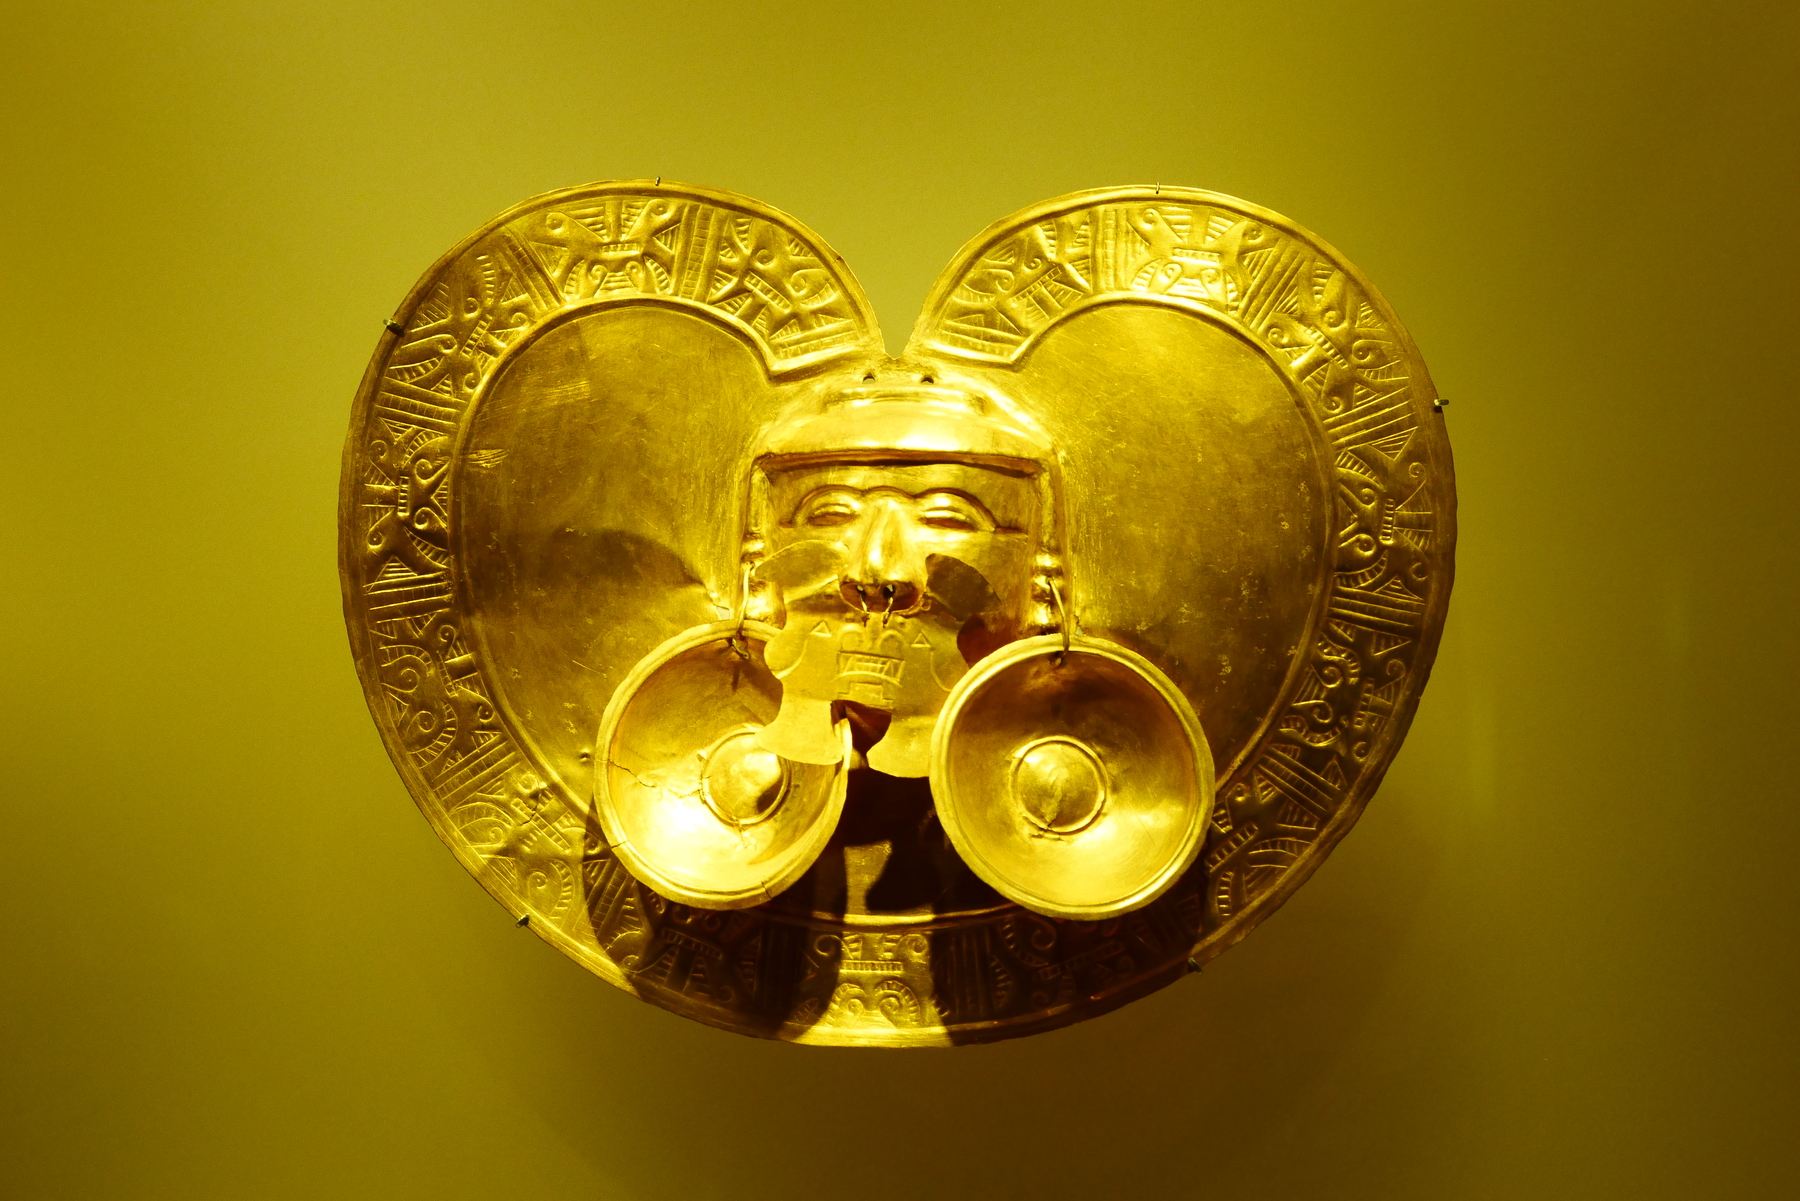
\includegraphics[height=95mm]{/home/ardila/Documents/pyLatexBook/scaled/P1110819.JPG}}%
}%
\caption{\texttt{[P1110819.JPG]} 04 January 2017}
\end{figure}

\vspace{8 mm}

\begin{figure}[ht!]
\centering
{%
\setlength{\fboxsep}{0pt}%
\setlength{\fboxrule}{0pt}%
\fbox{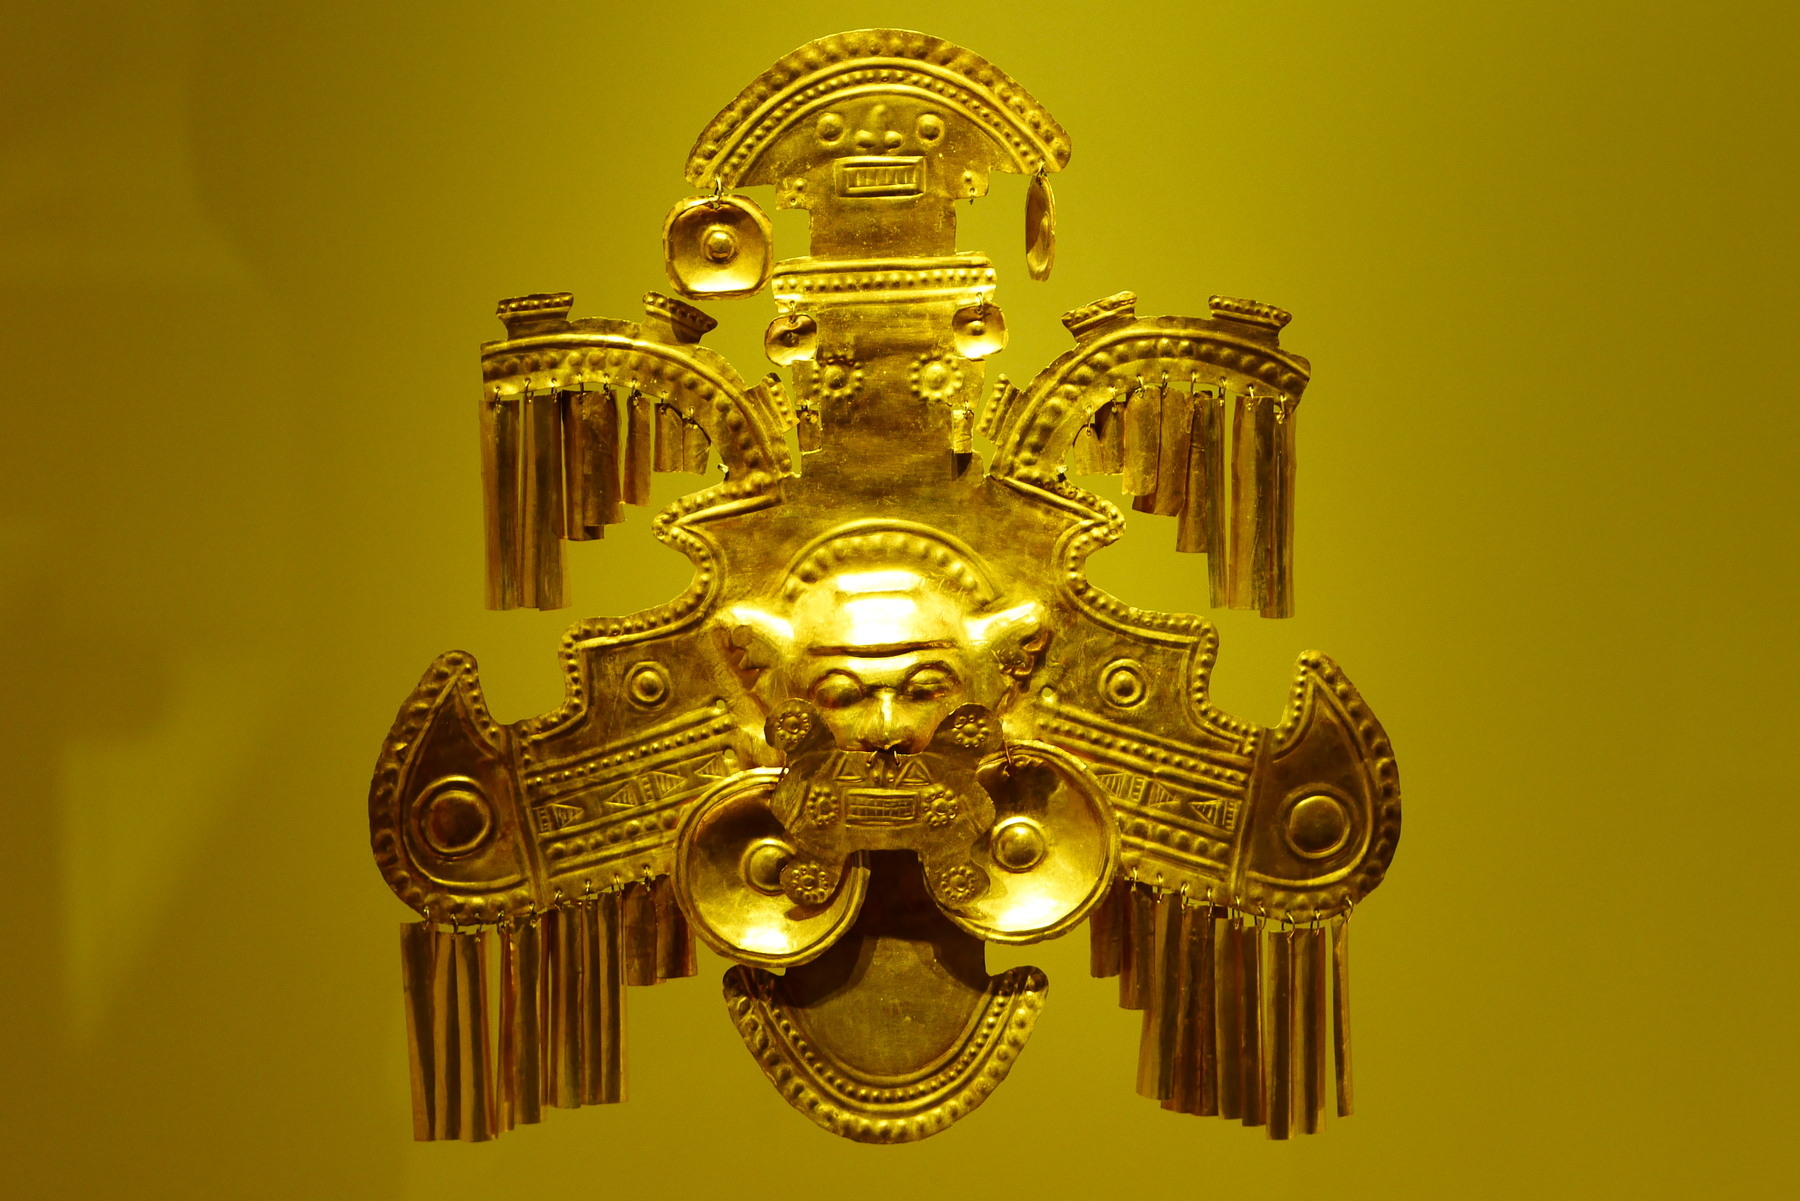
\includegraphics[height=95mm]{/home/ardila/Documents/pyLatexBook/scaled/P1110820.JPG}}%
}%
\caption{\texttt{[P1110820.JPG]} 04 January 2017}
\end{figure}

\newpage

\begin{figure}[ht!]
\centering
{%
\setlength{\fboxsep}{0pt}%
\setlength{\fboxrule}{0pt}%
\fbox{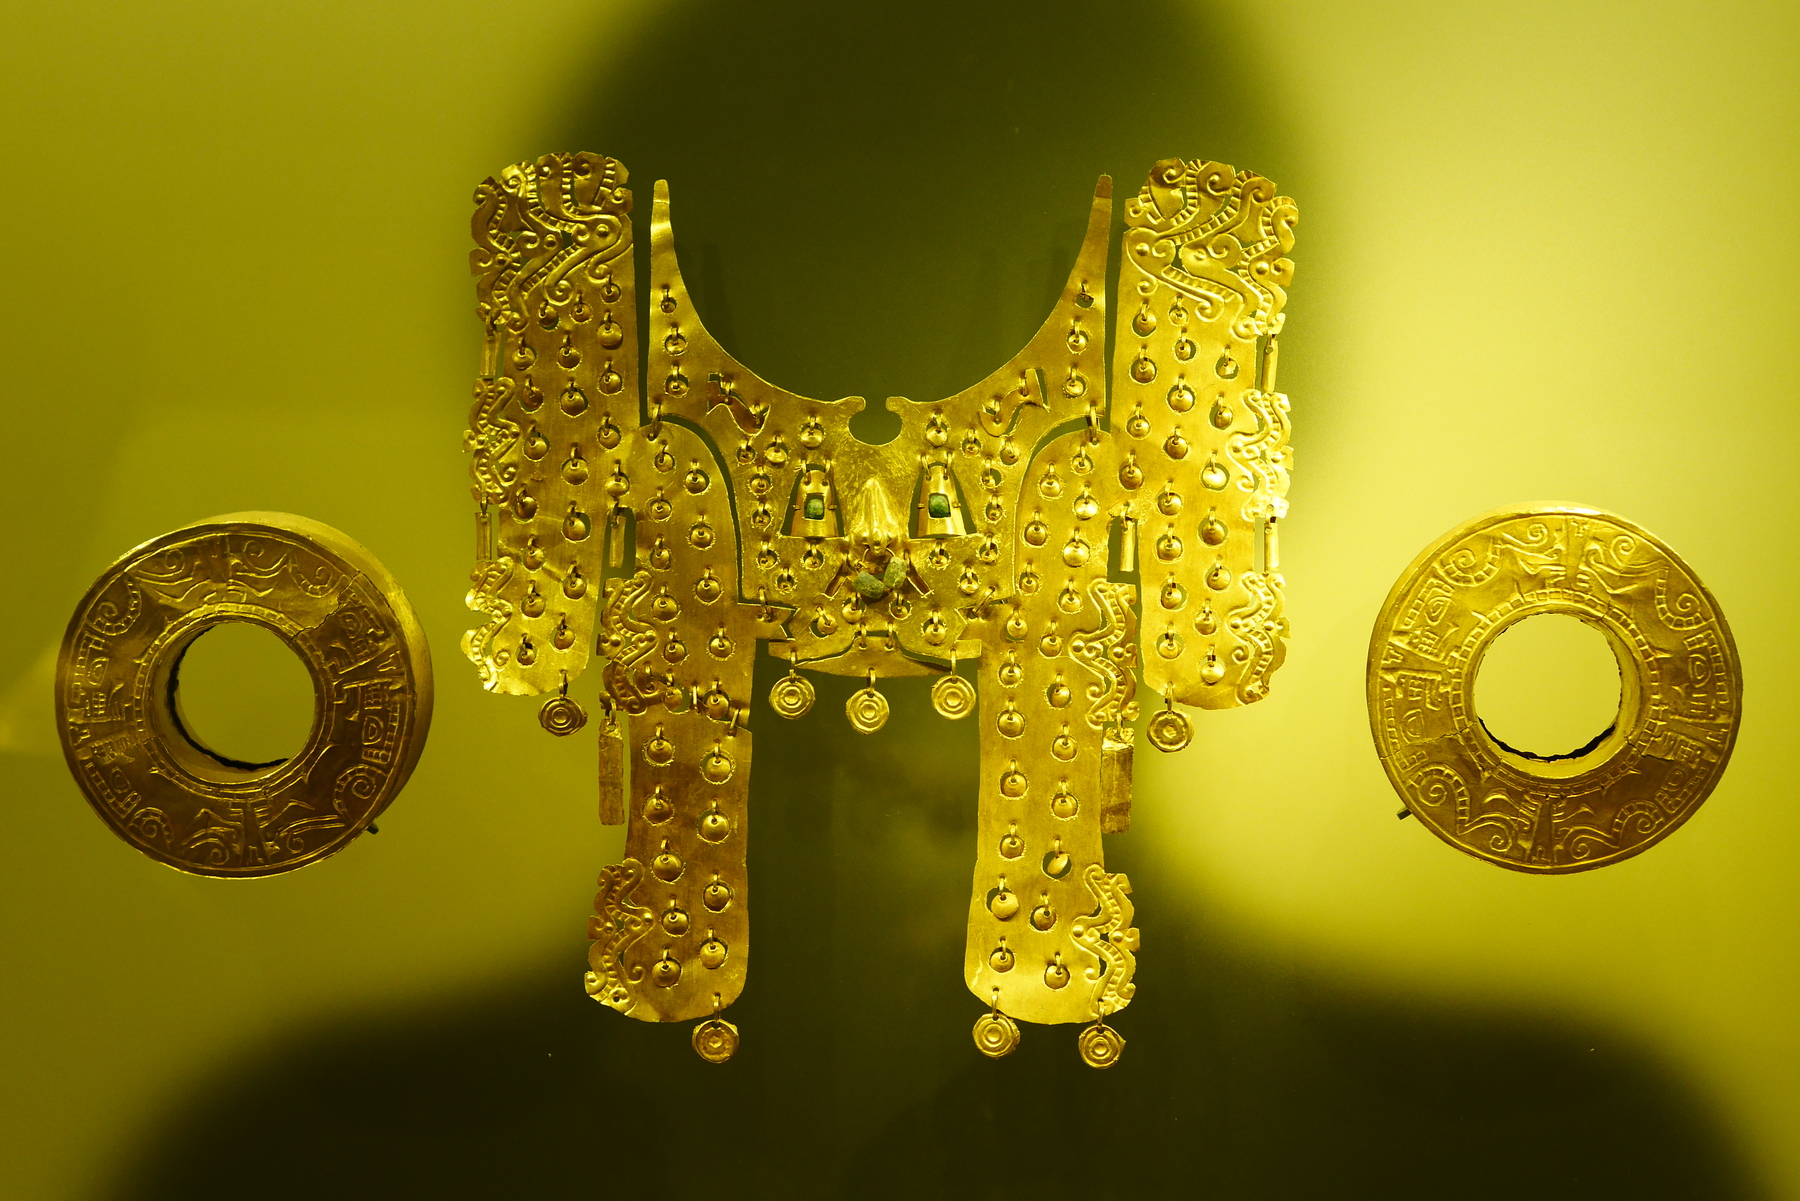
\includegraphics[height=95mm]{/home/ardila/Documents/pyLatexBook/scaled/P1110822.JPG}}%
}%
\caption{\texttt{[P1110822.JPG]} 04 January 2017}
\end{figure}

\vspace{8 mm}

\begin{figure}[ht!]
\centering
{%
\setlength{\fboxsep}{0pt}%
\setlength{\fboxrule}{0pt}%
\fbox{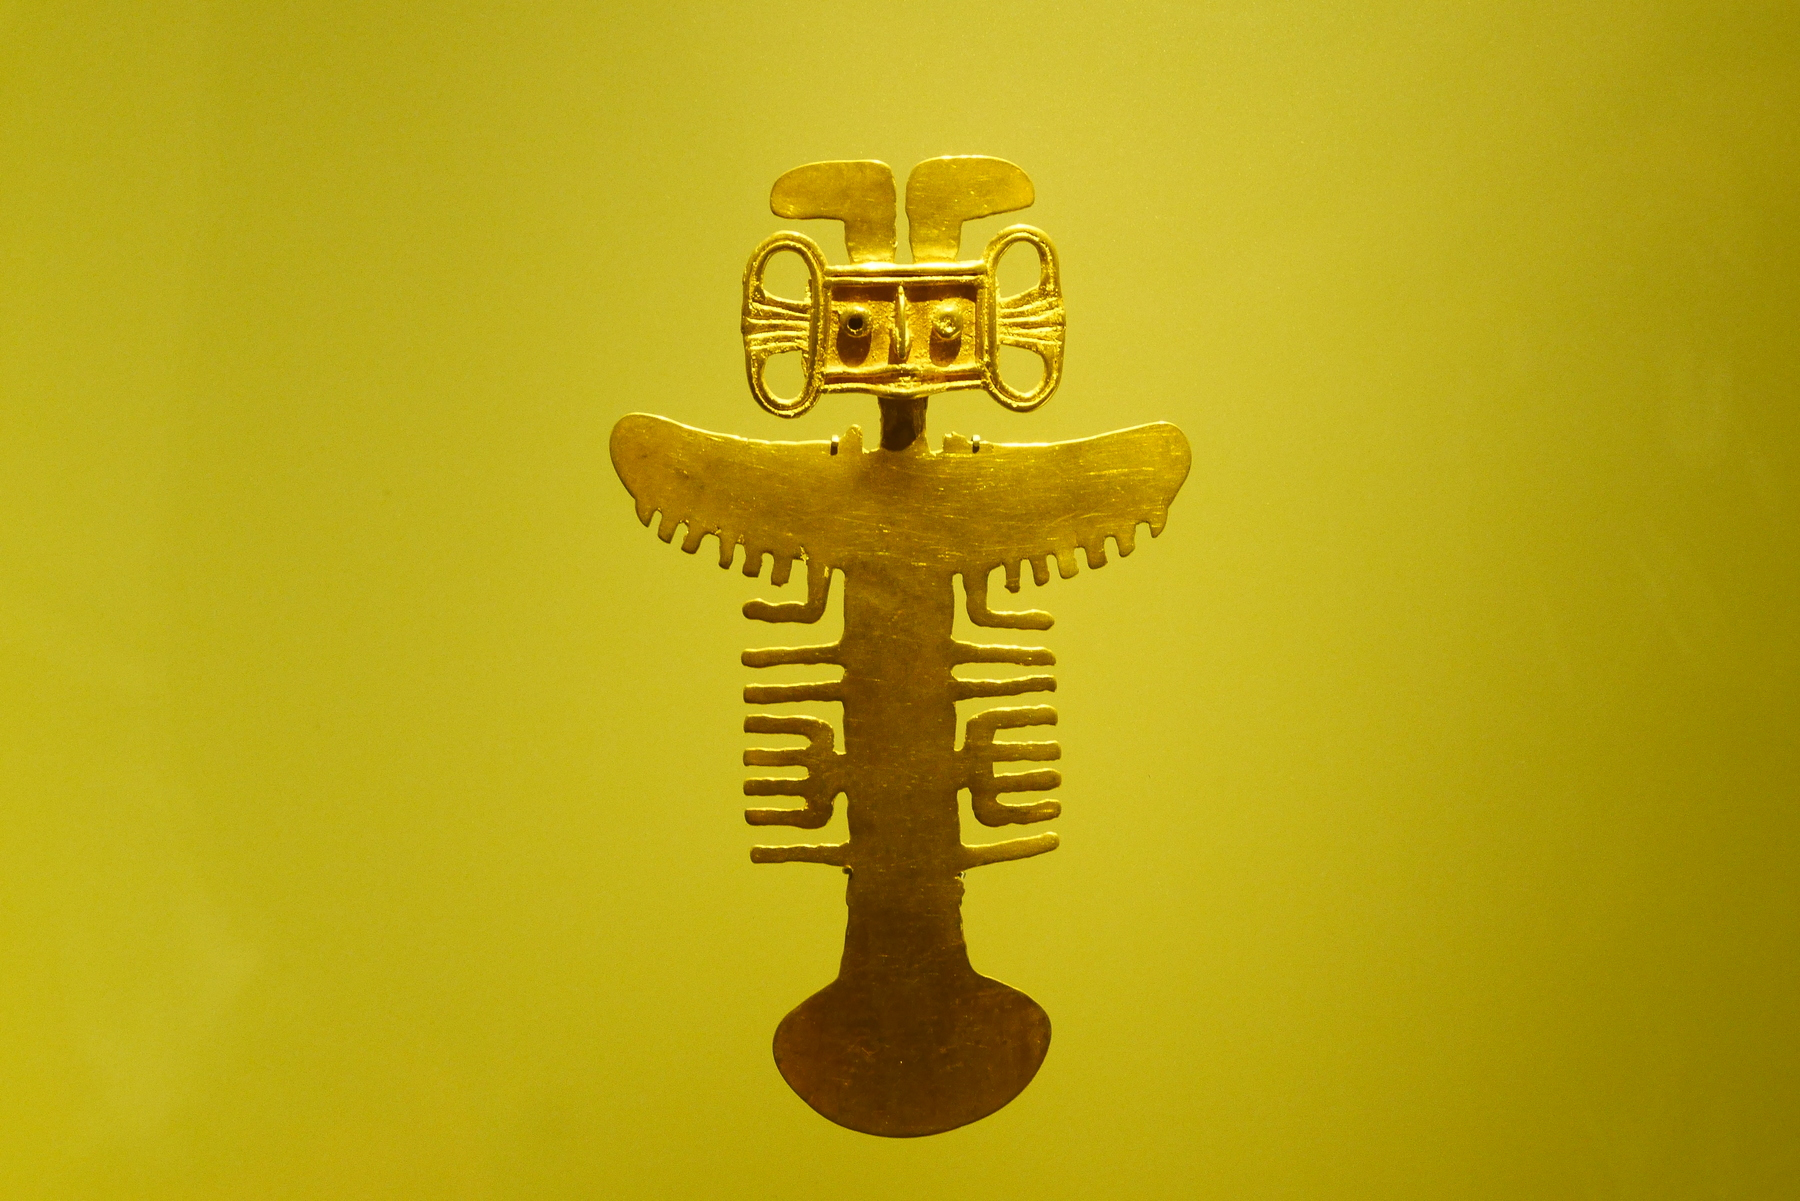
\includegraphics[height=95mm]{/home/ardila/Documents/pyLatexBook/scaled/P1110830.JPG}}%
}%
\caption{\texttt{[P1110830.JPG]} 04 January 2017}
\end{figure}

\newpage

\begin{figure}[ht!]
\centering
{%
\setlength{\fboxsep}{0pt}%
\setlength{\fboxrule}{0pt}%
\fbox{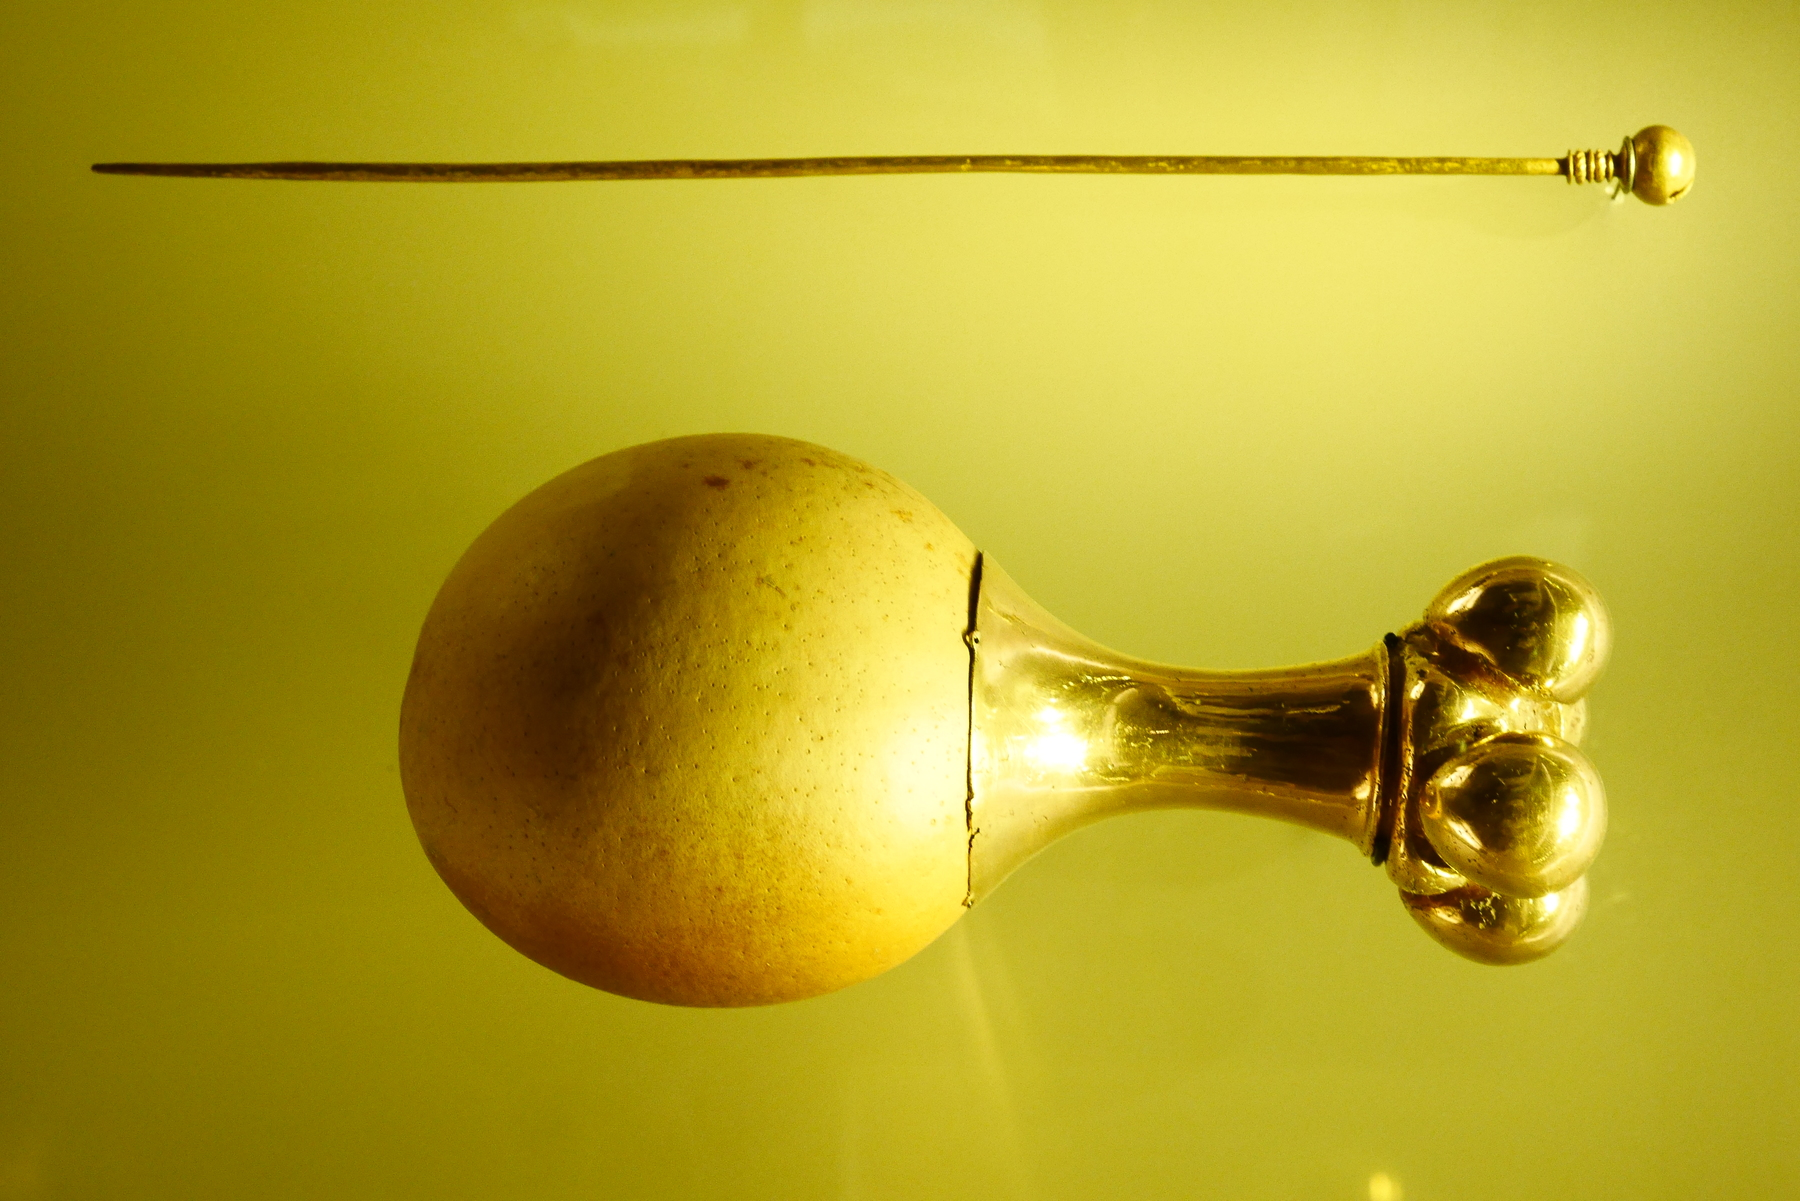
\includegraphics[height=95mm]{/home/ardila/Documents/pyLatexBook/scaled/P1110836.JPG}}%
}%
\caption{\texttt{[P1110836.JPG]} 04 January 2017}
\end{figure}

\vspace{8 mm}

\begin{figure}[ht!]
\centering
{%
\setlength{\fboxsep}{0pt}%
\setlength{\fboxrule}{0pt}%
\fbox{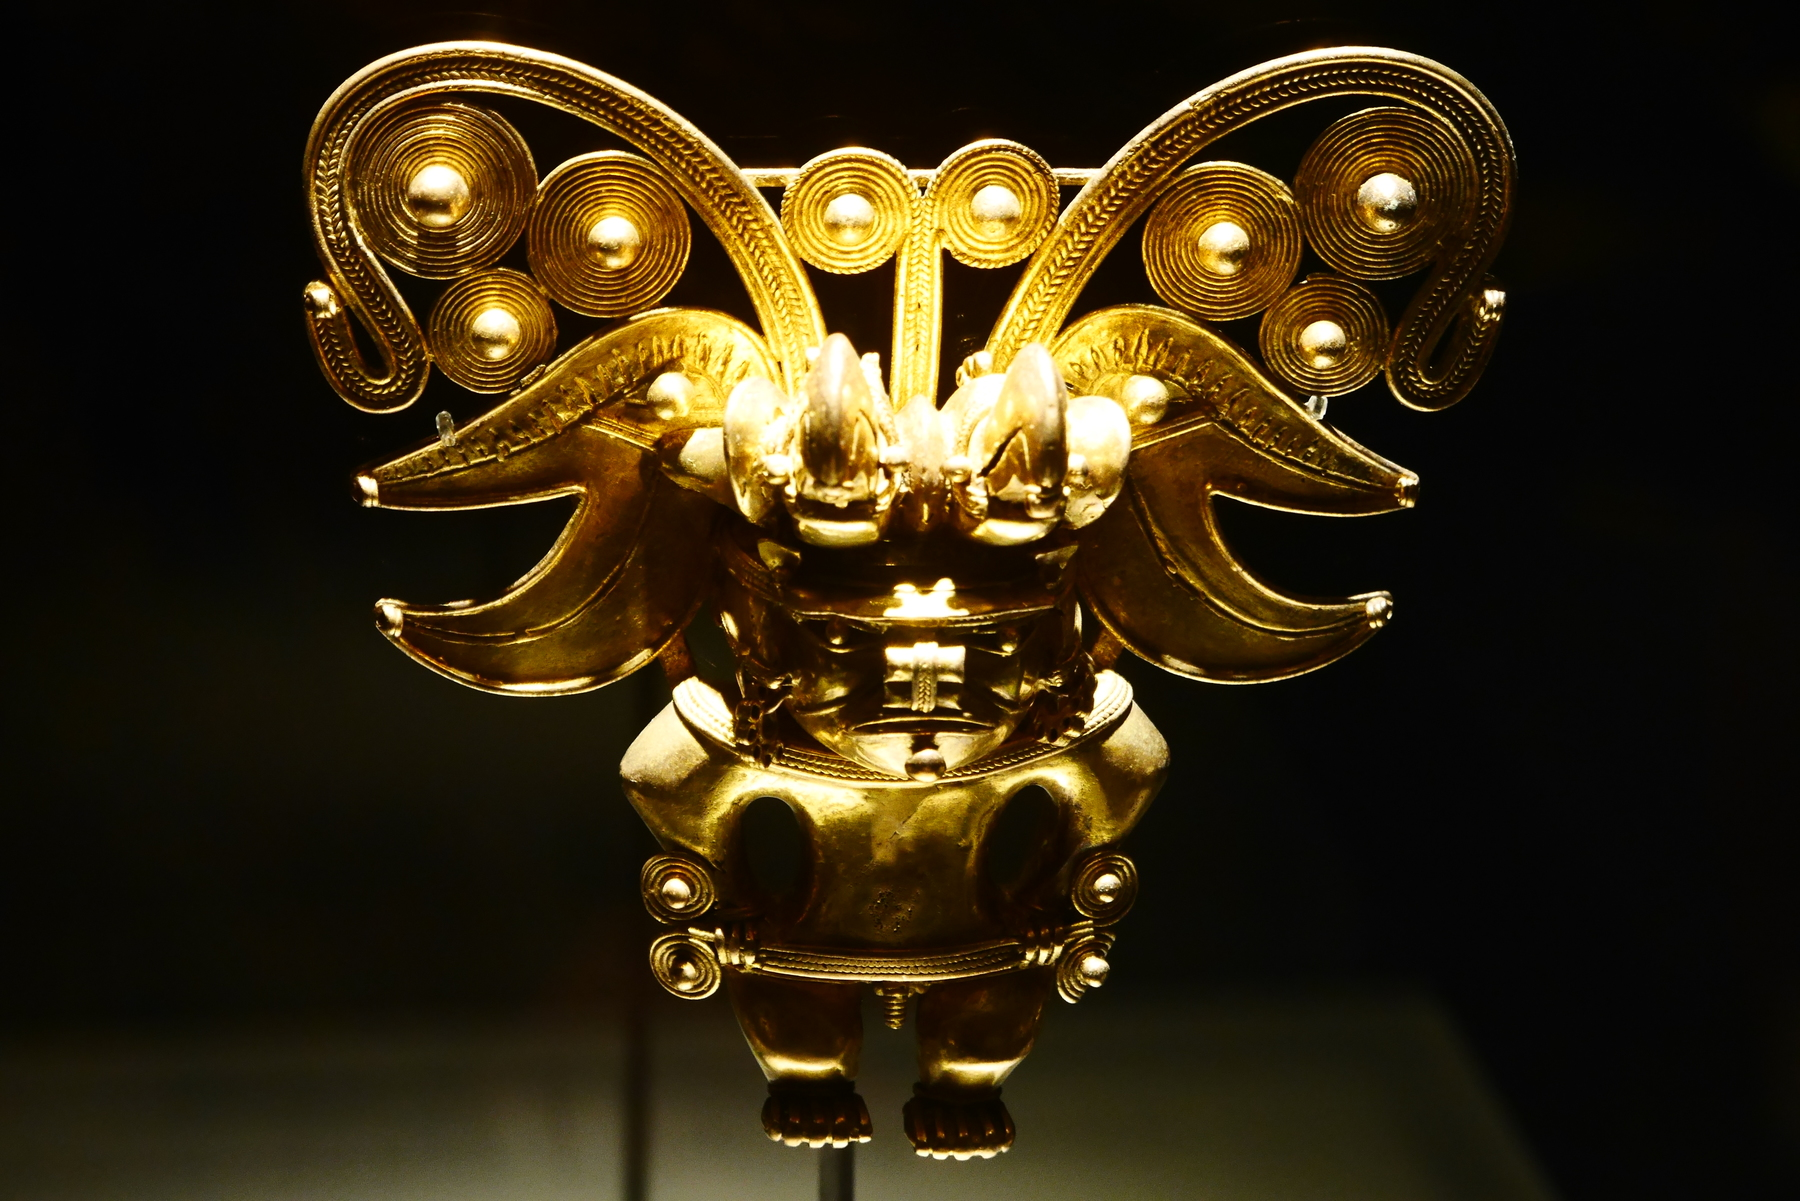
\includegraphics[height=95mm]{/home/ardila/Documents/pyLatexBook/scaled/P1110864.JPG}}%
}%
\caption{\texttt{[P1110864.JPG]} 04 January 2017}
\end{figure}

\newpage

\begin{figure}[ht!]
\centering
{%
\setlength{\fboxsep}{0pt}%
\setlength{\fboxrule}{0pt}%
\fbox{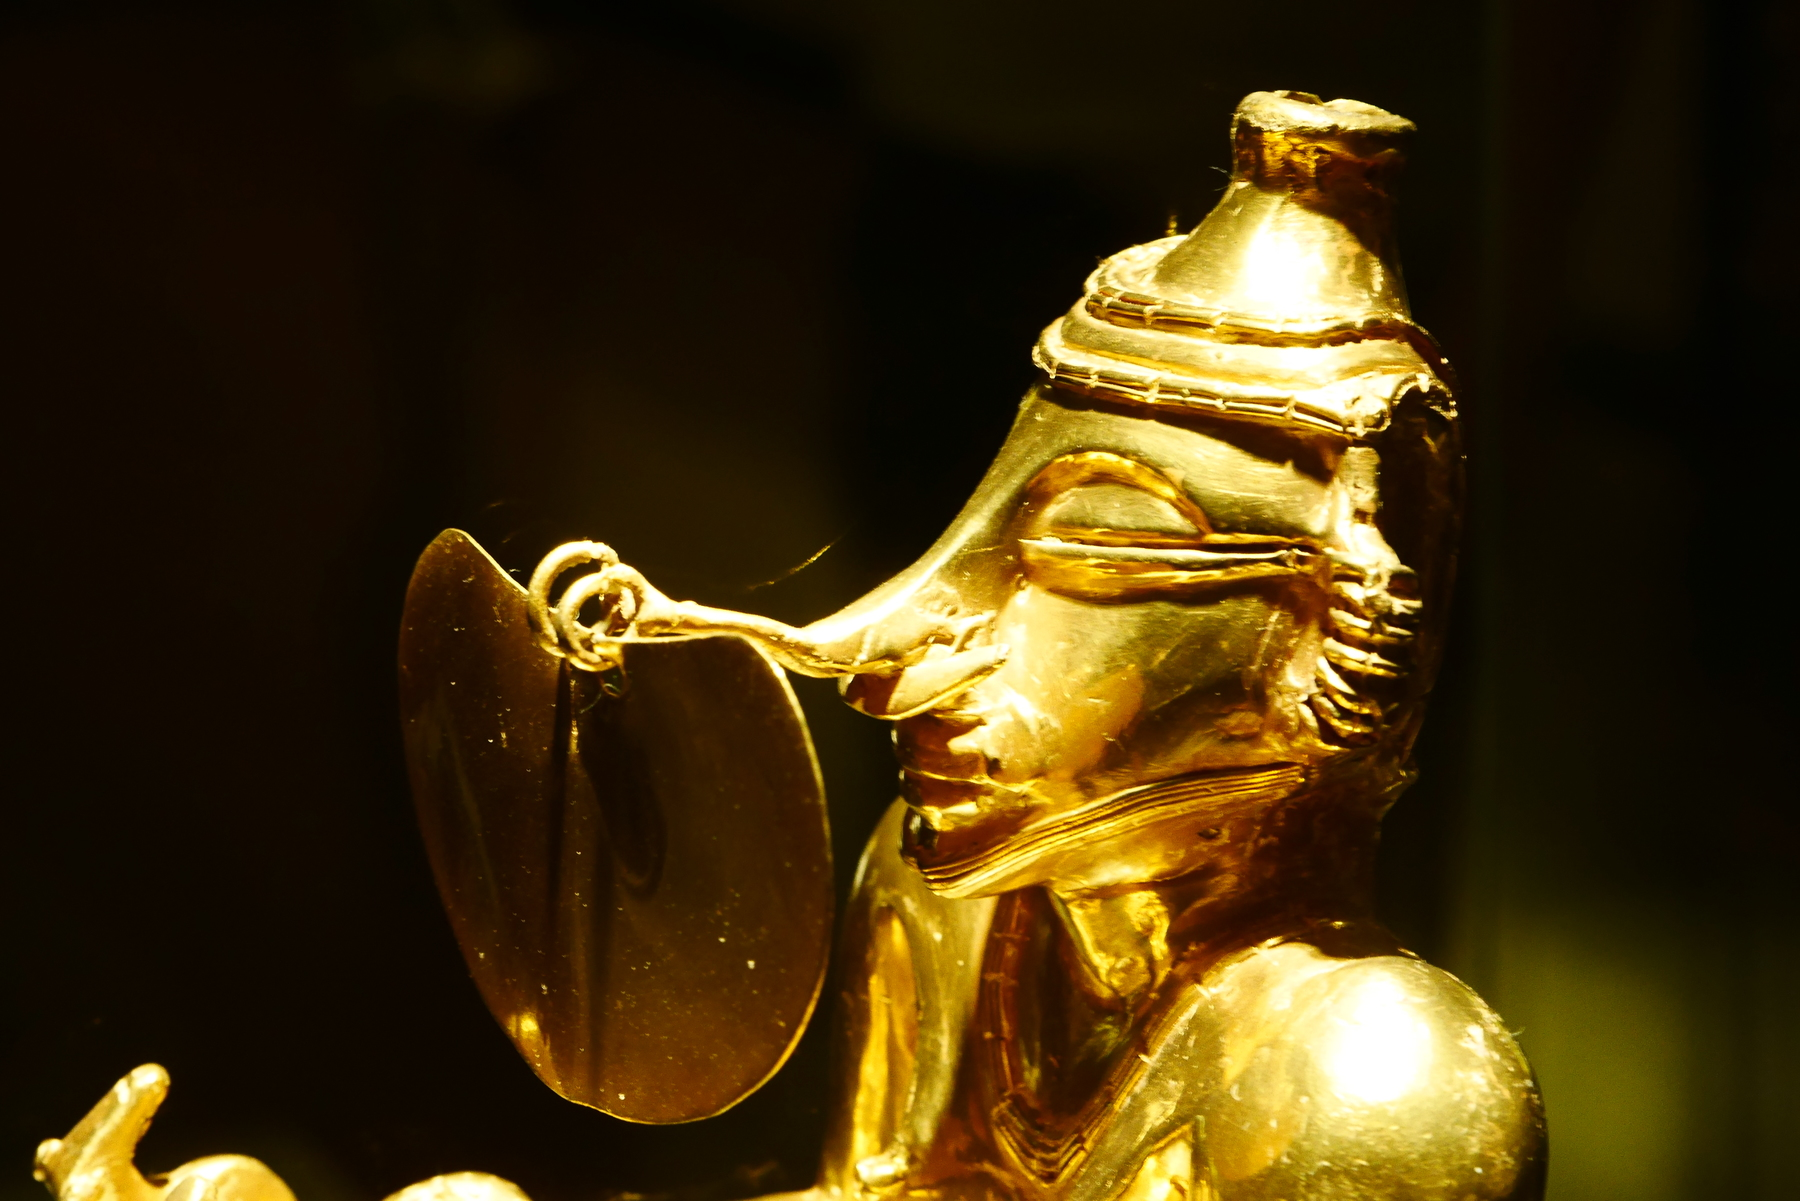
\includegraphics[height=95mm]{/home/ardila/Documents/pyLatexBook/scaled/P1110869.JPG}}%
}%
\caption{\texttt{[P1110869.JPG]} 04 January 2017}
\end{figure}

\vspace{8 mm}

\begin{figure}[ht!]
\centering
{%
\setlength{\fboxsep}{0pt}%
\setlength{\fboxrule}{0pt}%
\fbox{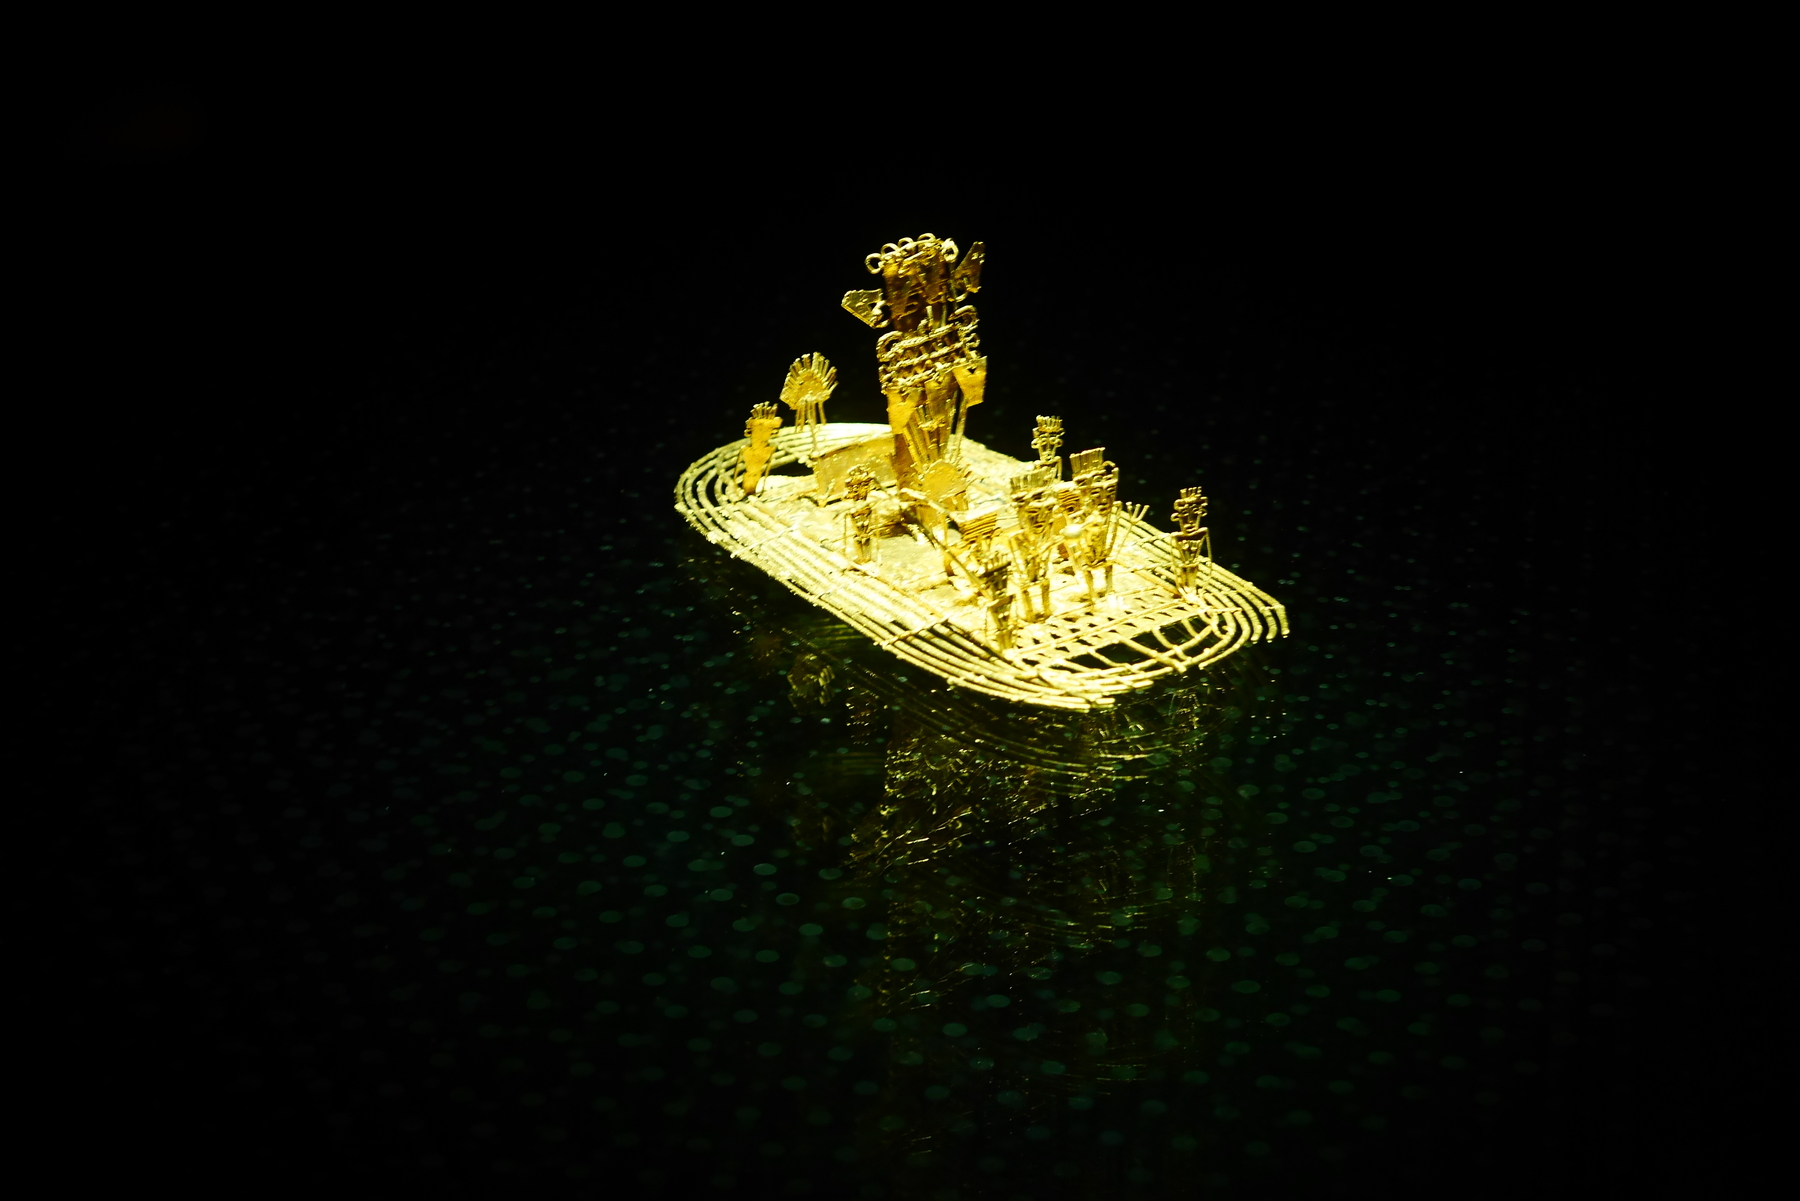
\includegraphics[height=95mm]{/home/ardila/Documents/pyLatexBook/scaled/P1110877.JPG}}%
}%
\caption{\texttt{[P1110877.JPG]} 04 January 2017}
\end{figure}

\newpage

\begin{figure}[ht!]
\centering
{%
\setlength{\fboxsep}{0pt}%
\setlength{\fboxrule}{0pt}%
\fbox{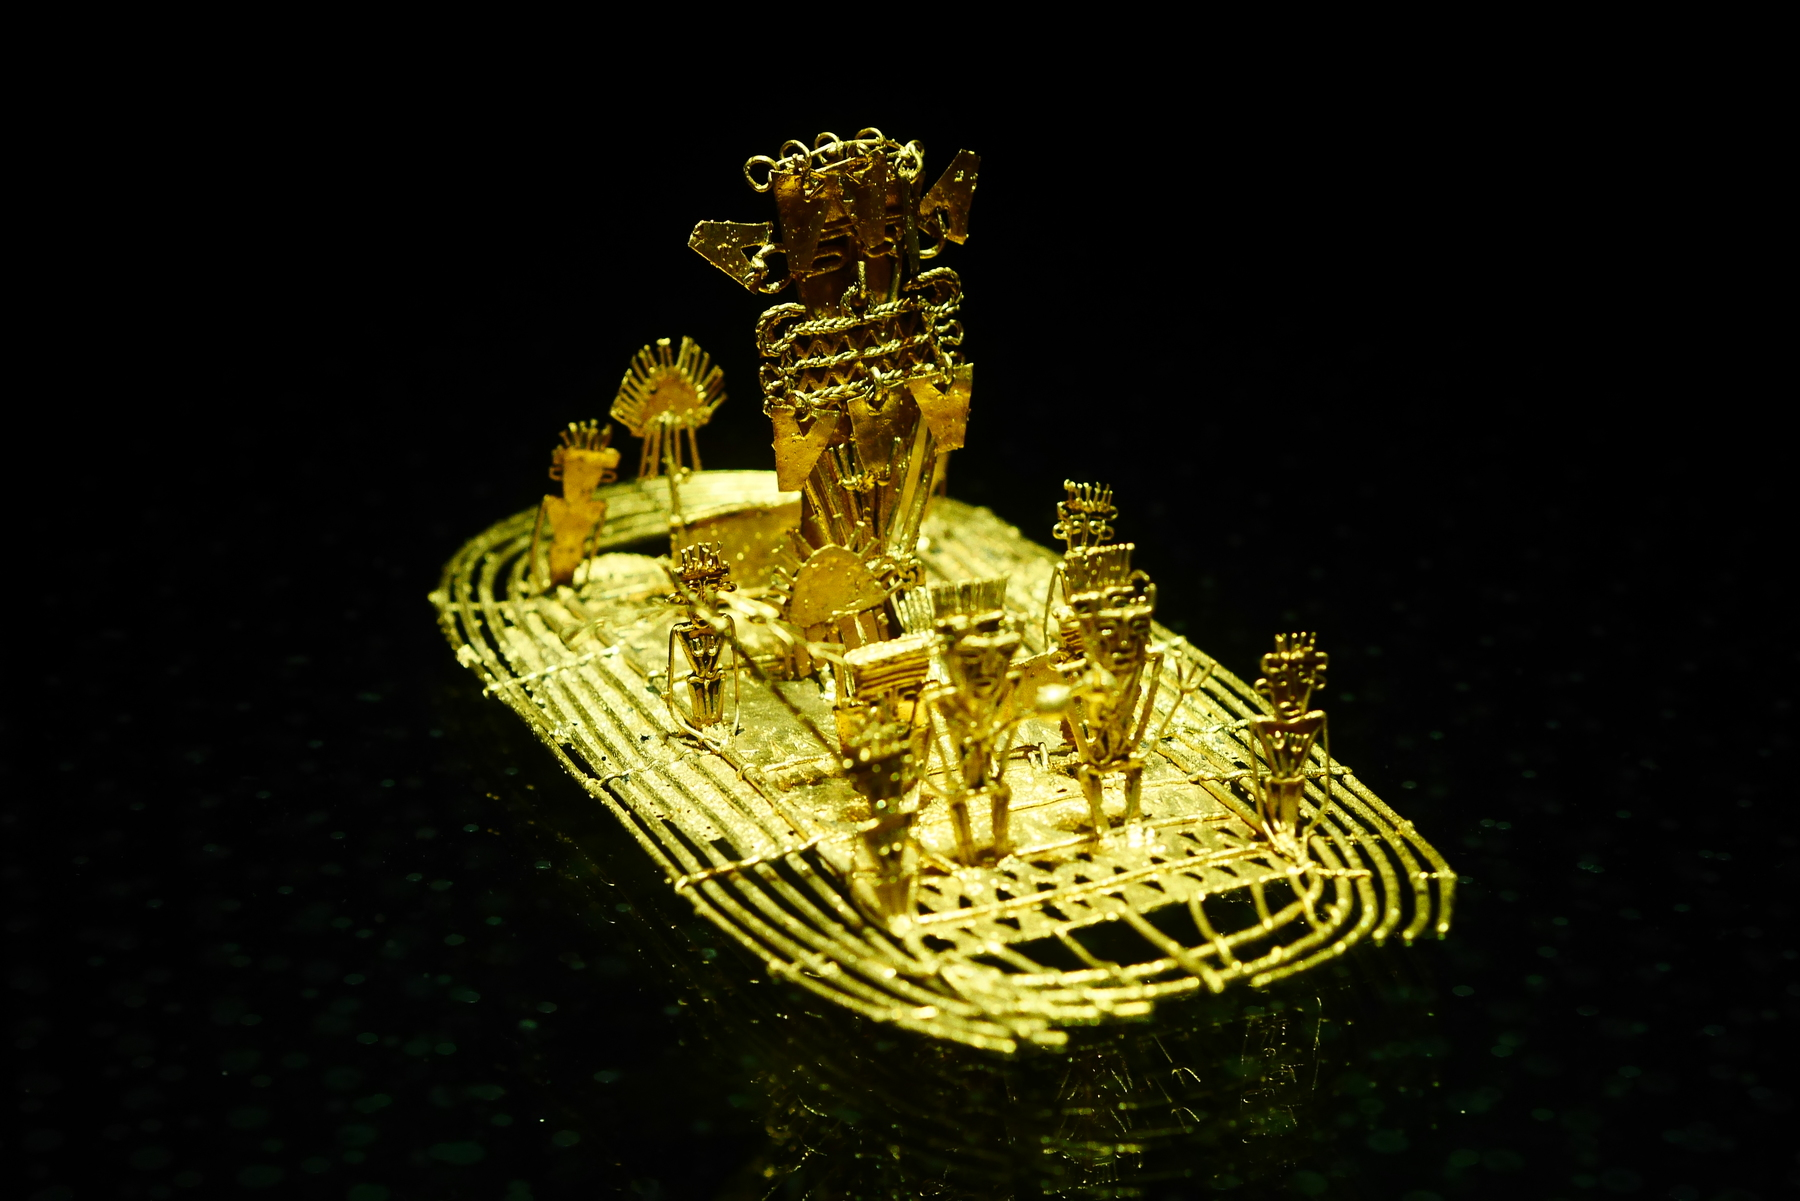
\includegraphics[height=95mm]{/home/ardila/Documents/pyLatexBook/scaled/P1110880.JPG}}%
}%
\caption{\texttt{[P1110880.JPG]} 04 January 2017}
\end{figure}

\vspace{8 mm}

\begin{figure}[ht!]
\centering
{%
\setlength{\fboxsep}{0pt}%
\setlength{\fboxrule}{0pt}%
\fbox{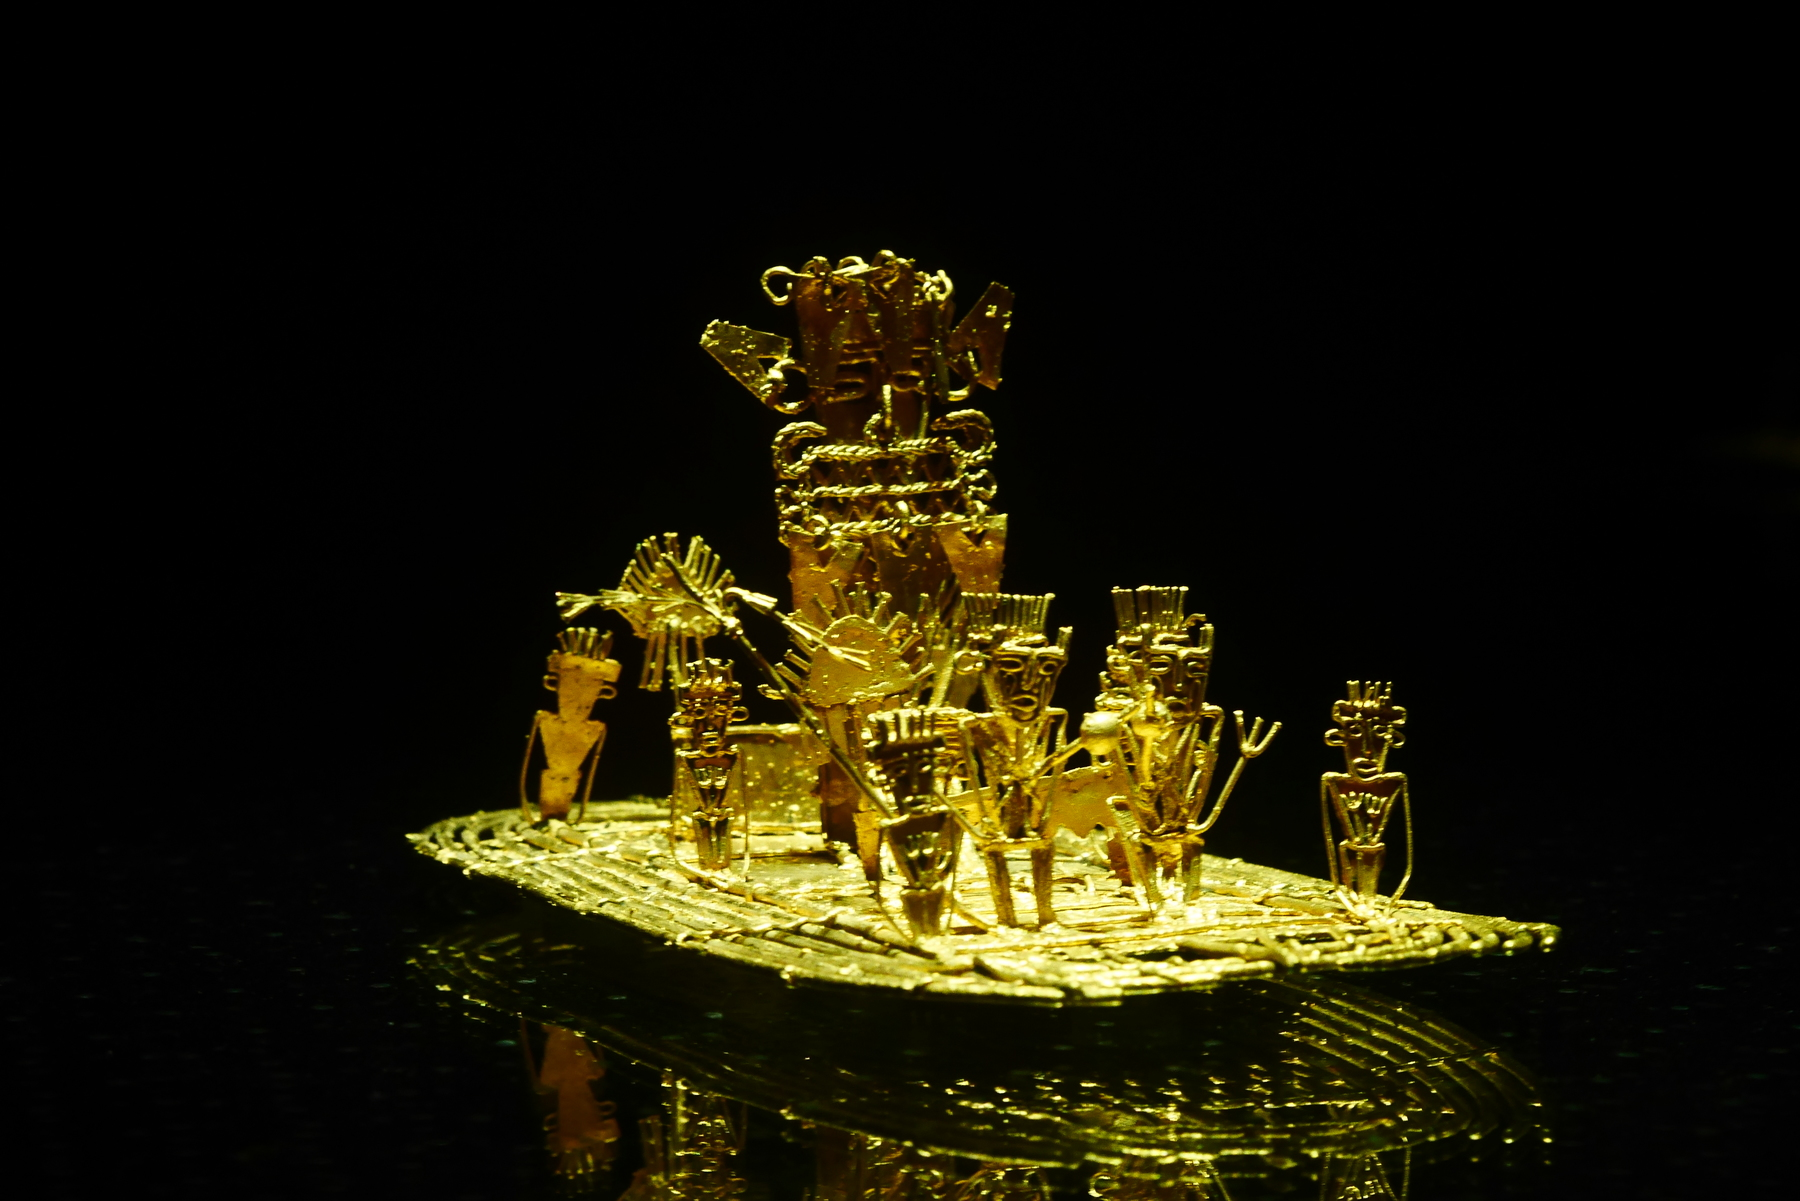
\includegraphics[height=95mm]{/home/ardila/Documents/pyLatexBook/scaled/P1110888.JPG}}%
}%
\caption{\texttt{[P1110888.JPG]} 04 January 2017}
\end{figure}

\newpage

\begin{figure}[ht!]
\centering
{%
\setlength{\fboxsep}{0pt}%
\setlength{\fboxrule}{0pt}%
\fbox{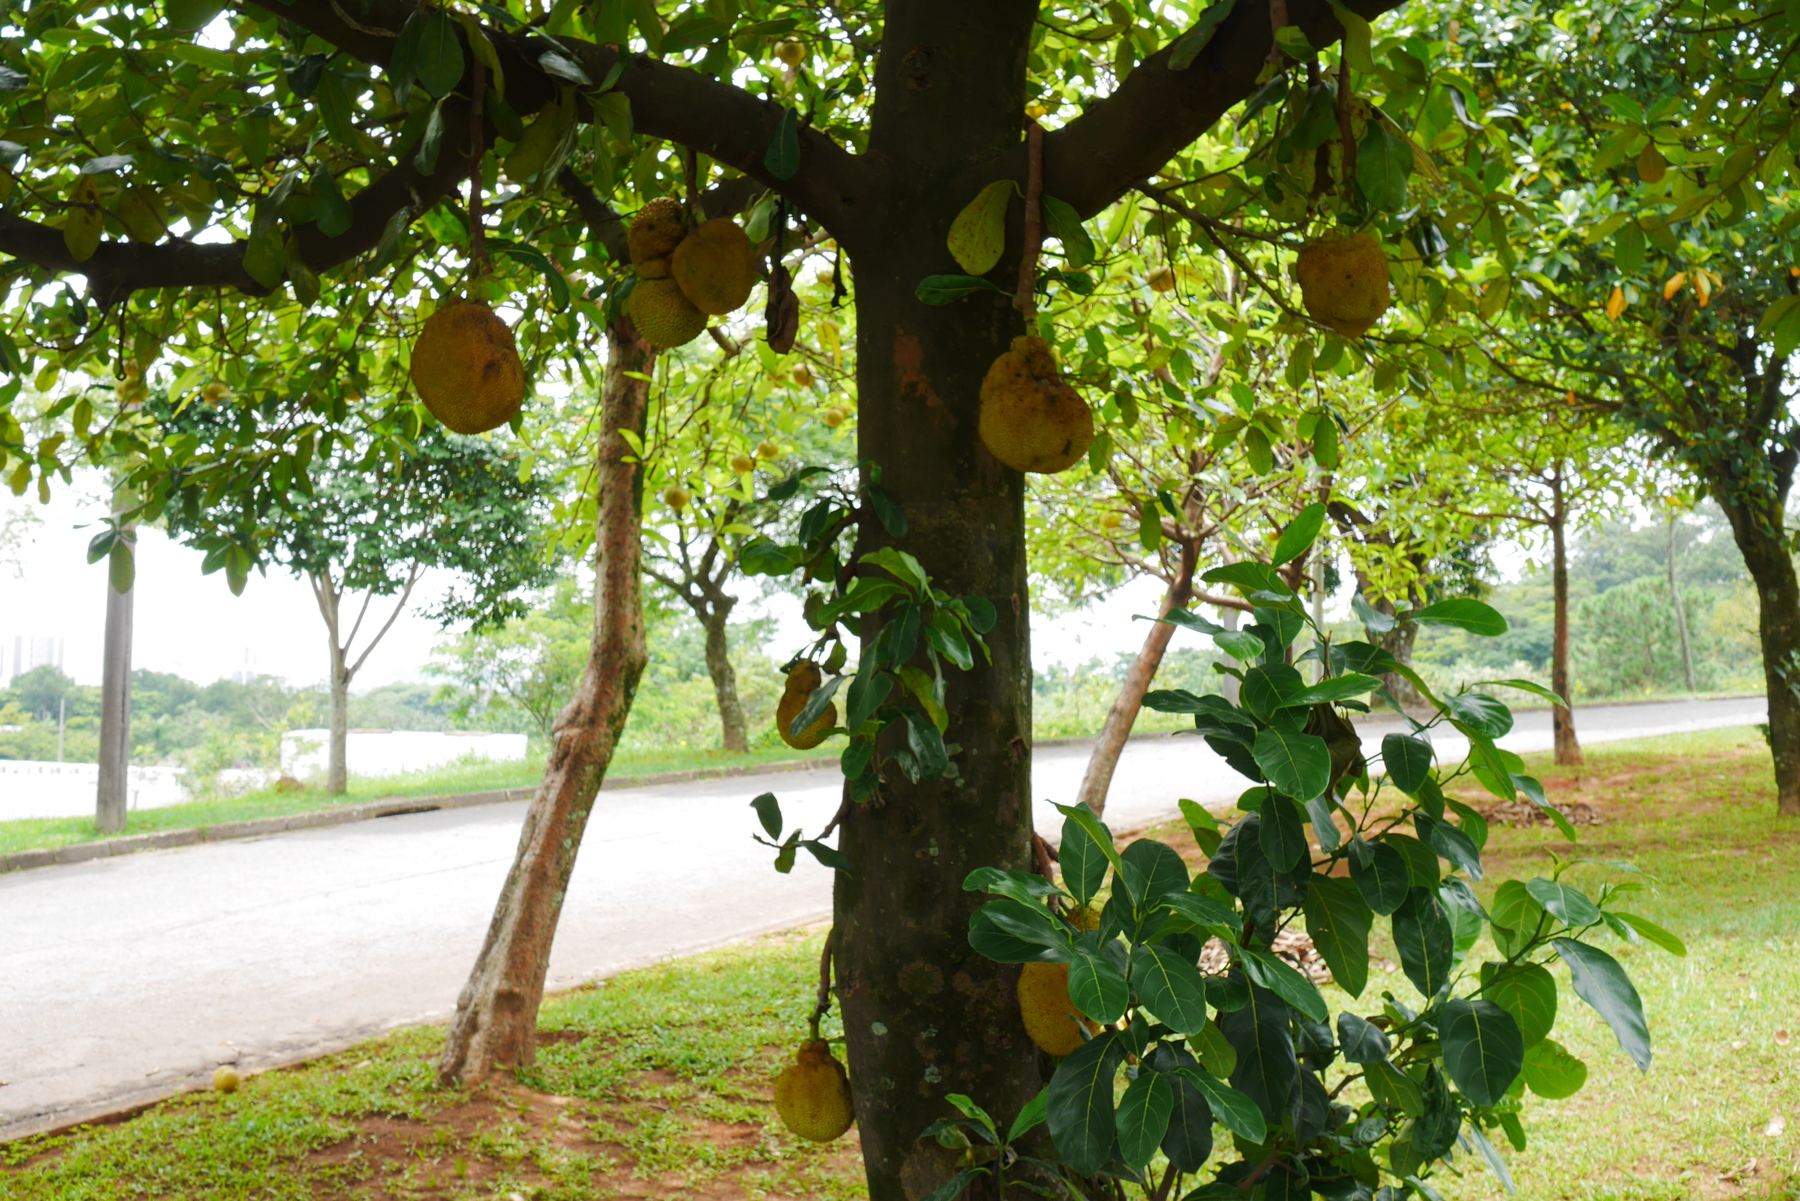
\includegraphics[height=95mm]{/home/ardila/Documents/pyLatexBook/scaled/P1120751.JPG}}%
}%
\caption{\texttt{[P1120751.JPG]} 31 January 2017}
\end{figure}

\vspace{8 mm}

\begin{figure}[ht!]
\centering
{%
\setlength{\fboxsep}{0pt}%
\setlength{\fboxrule}{0pt}%
\fbox{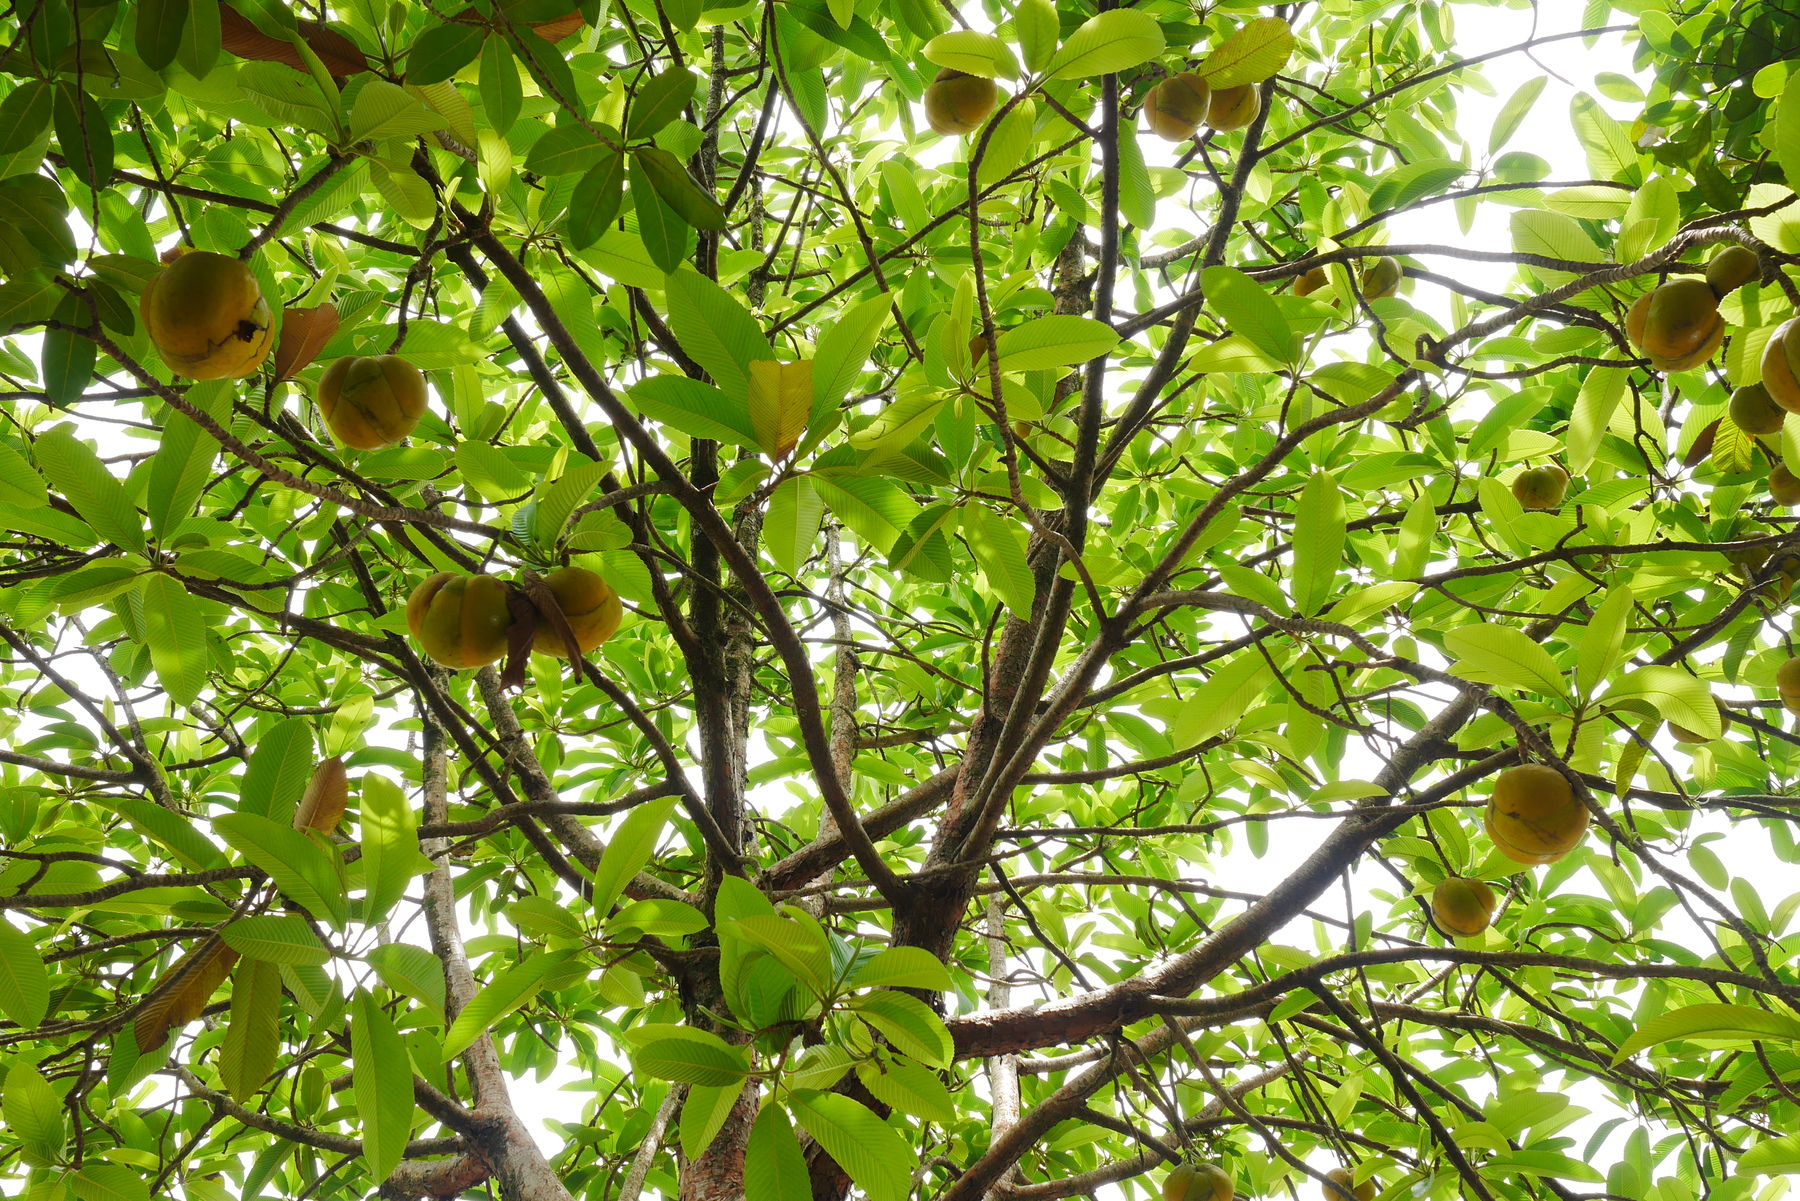
\includegraphics[height=95mm]{/home/ardila/Documents/pyLatexBook/scaled/P1120752.JPG}}%
}%
\caption{\texttt{[P1120752.JPG]} 31 January 2017}
\end{figure}

\newpage

\begin{figure}[ht!]
\centering
{%
\setlength{\fboxsep}{0pt}%
\setlength{\fboxrule}{0pt}%
\fbox{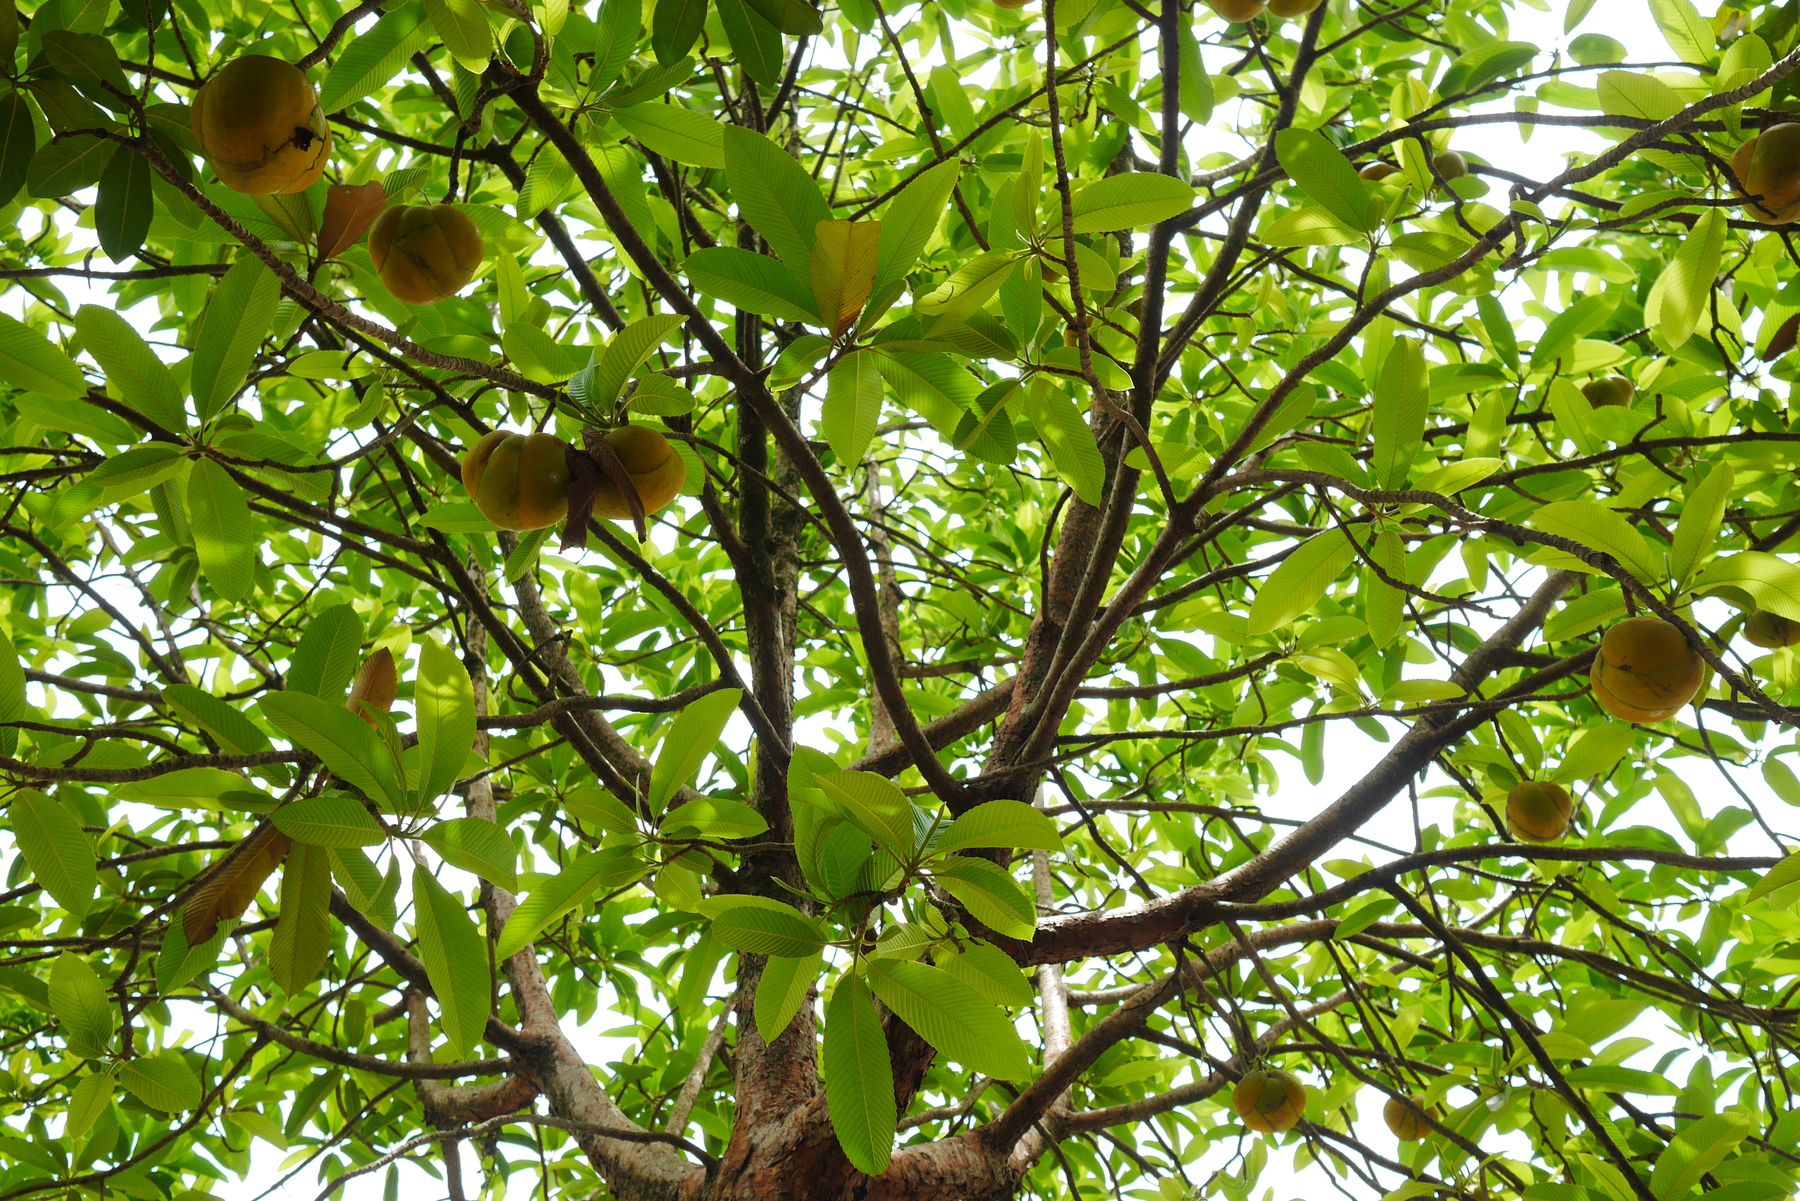
\includegraphics[height=95mm]{/home/ardila/Documents/pyLatexBook/scaled/P1120753.JPG}}%
}%
\caption{\texttt{[P1120753.JPG]} 31 January 2017}
\end{figure}

\vspace{8 mm}

\begin{figure}[ht!]
\centering
{%
\setlength{\fboxsep}{0pt}%
\setlength{\fboxrule}{0pt}%
\fbox{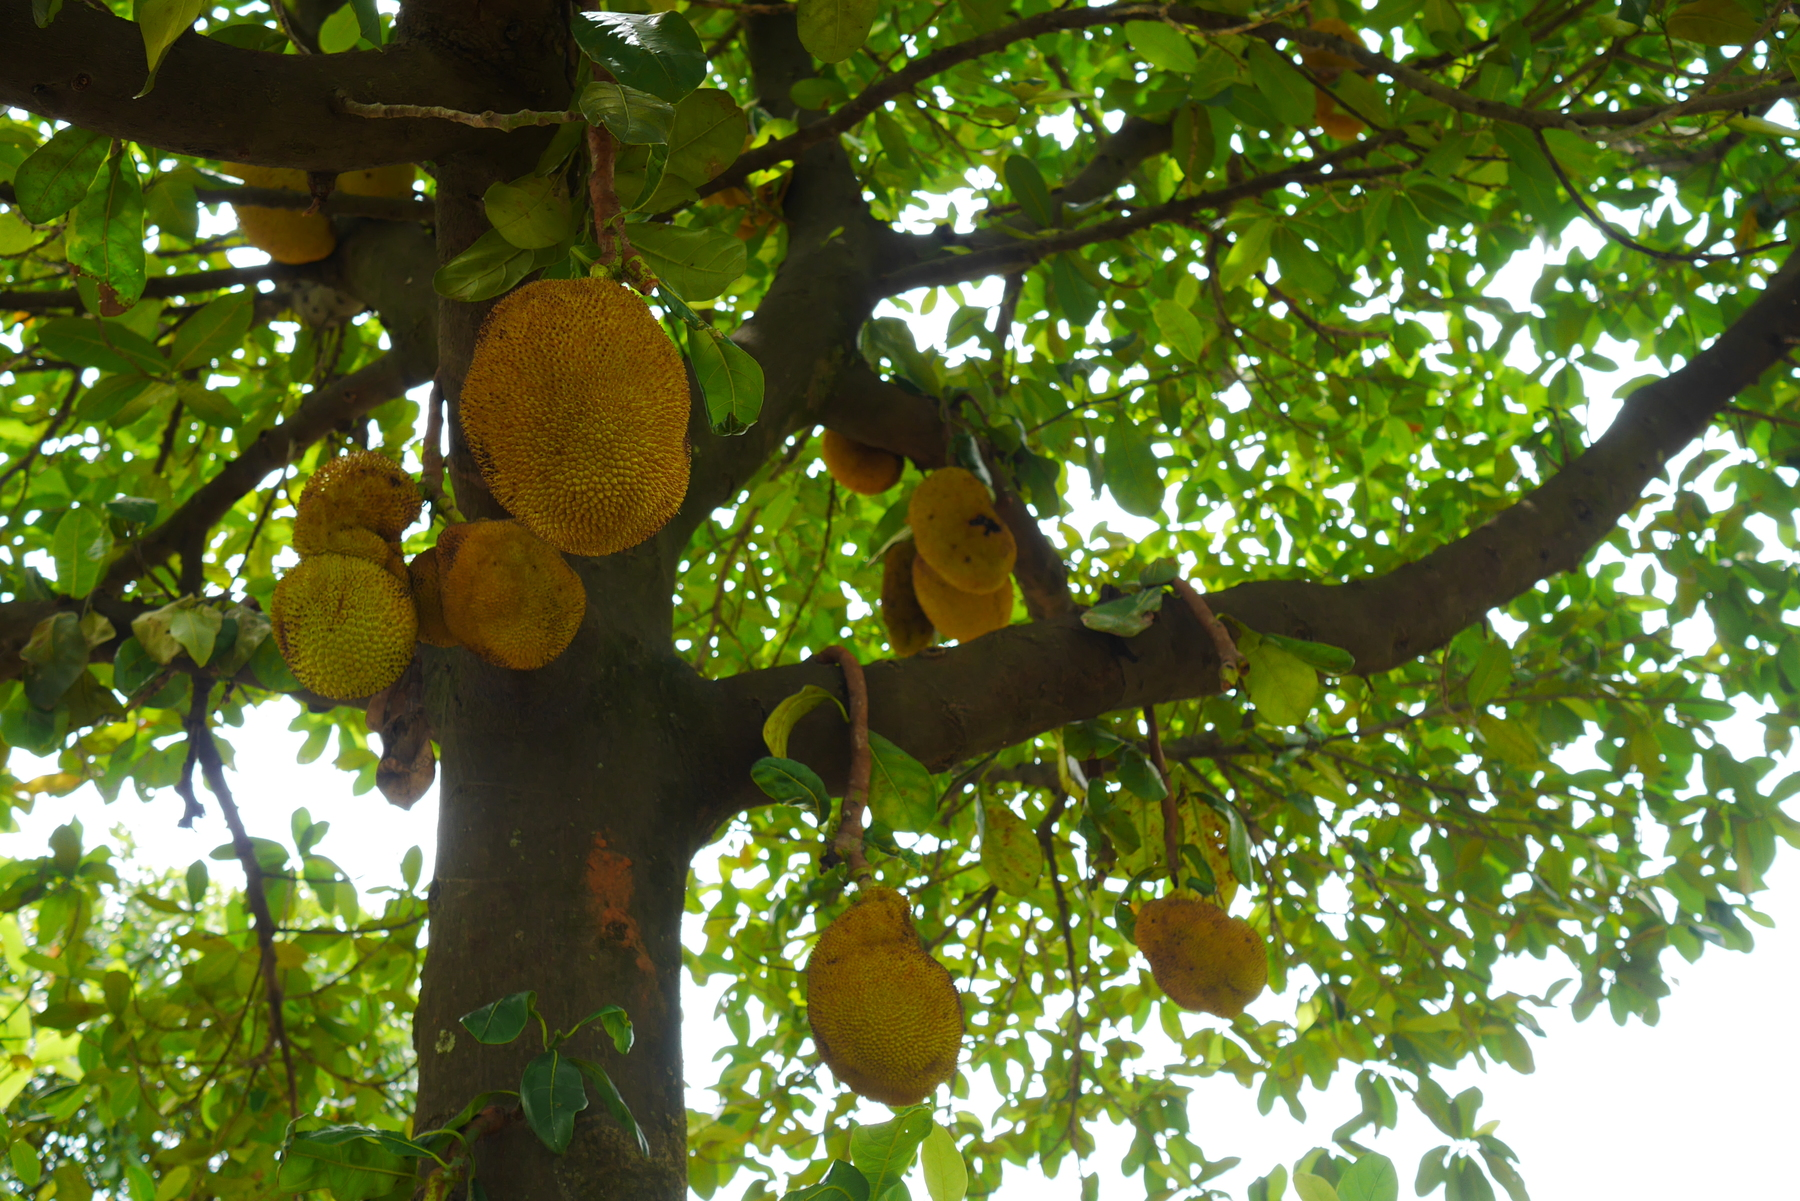
\includegraphics[height=95mm]{/home/ardila/Documents/pyLatexBook/scaled/P1120754.JPG}}%
}%
\caption{\texttt{[P1120754.JPG]} 31 January 2017}
\end{figure}

\newpage



\end{document}


